\documentclass{article}
\usepackage[utf8]{inputenc}
\usepackage[english]{babel}
\usepackage{amssymb}
\usepackage{amsmath}
\usepackage{amsthm}
\usepackage{color}
\usepackage{todonotes}
\usepackage{mathtools}
\usepackage{etoolbox}
\usepackage{float}
%\usepackage{showkeys}
\usepackage[a4paper, total={6.5in, 9in}]{geometry}
\usepackage{graphicx}
\usepackage[center]{subfigure}

\usetikzlibrary{shapes.geometric, arrows,backgrounds,fit}
\usetikzlibrary{decorations.pathreplacing}


\tikzstyle{block} = [rectangle, rounded corners, minimum height=1cm,text centered, draw=black]
\tikzstyle{arrow} = [thick,->,>=stealth]
\tikzstyle{edgered} = [red,thick]
\tikzstyle{edgeblue} = [blue,thick]
\tikzstyle{edgegreen} = [green,thick]

\pgfdeclarelayer{bg}    % declare background layer
\pgfsetlayers{bg,main}  % set the order of the layers (main is the standard layer)

\tikzset{neuron/.style={circle,draw,minimum size=4mm,line width = 1pt},neuron missing/.style={draw=none, scale=1.5,text height=2mm,execute at begin node=\color{black}$\vdots$}}


\begin{document}

\begin{minipage}{0.45\linewidth}
\begin{figure}[H]
    \centering
    \resizebox{1\textwidth}{!}{%
    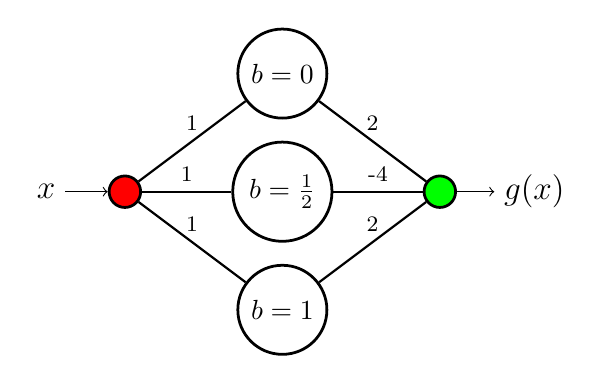
\begin{tikzpicture}
    \node [neuron, draw = black, fill = red] (input1) at (0,0) {} ;
    \node [neuron, right of = input1, yshift = 0cm, xshift = 1cm, fill=white] (hidden12) {$b=\frac{1}{2}$};
    \node [neuron, above of = hidden12, yshift = .5cm, xshift = 0cm, fill=white] (hidden11) { $b=0$};
    \node [neuron, below of = hidden12, yshift = -.5cm, fill=white] (hidden13) {$b=1$};

    \node [neuron, right of = hidden12, yshift = 0cm, xshift = 1cm, draw = black, fill = green] (output) {};

    \begin{pgfonlayer}{bg} % background layer
    \draw[thick] (input1) -- (hidden11) node[midway, above] {\footnotesize 1};
    \draw[thick] (input1) -- (hidden12) node[midway, above] {\footnotesize 1};
    \draw[thick] (input1) -- (hidden13) node[midway, above] {\footnotesize 1};
    \draw[thick] (hidden11) -- (output) node[midway, above] {\footnotesize 2};
    \draw[thick] (hidden12) -- (output) node[midway, above] {\footnotesize -4};
    \draw[thick] (hidden13) -- (output) node[midway, above] {\footnotesize 2};
    \end{pgfonlayer}
        
    \node [draw = none, left of = input1] (inputlabel1) {\large $x$};
    \draw [->] (inputlabel1) --  (input1);
    \node [draw = none, right of = output, xshift = 0.2cm] (outputlabel) {\large $g(x)$};
    \draw [->] (output) --  (outputlabel);
    \end{tikzpicture}
    }%
    % \caption{.}
    % \label{.}
\end{figure}
\end{minipage}
\hspace{0.05\linewidth}
\begin{minipage}{0.45\linewidth}
\begin{figure}[H]
    \centering
    \resizebox{1\textwidth}{!}{%
    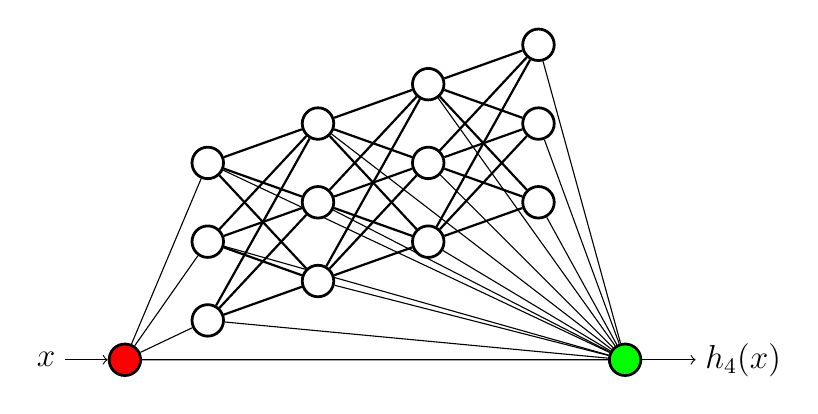
\begin{tikzpicture}
    \node [neuron, draw = black, fill = red] (input1) at (0,0) {} ;
    \node [neuron, right of = input1, yshift = 2.5cm, xshift = 1.5, fill=white] (hidden11) {};
    \node [neuron, below of = hidden11, yshift = 0cm, fill=white] (hidden12) {};
    \node [neuron, below of = hidden12, yshift = 0cm, fill=white] (hidden13) {};

    \node [neuron, right of = hidden11, yshift = 0.5cm, xshift = .4cm, fill=white] (hidden21) {};
    \node [neuron, below of = hidden21, yshift = 0cm, fill=white] (hidden22) {};
    \node [neuron, below of = hidden22, yshift = 0cm, fill=white] (hidden23) {};

    \node [neuron, right of = hidden21, yshift = 0.5cm, xshift = .4cm, fill=white] (hidden31) {};
    \node [neuron, below of = hidden31, yshift = 0cm, fill=white] (hidden32) {};
    \node [neuron, below of = hidden32, yshift = 0cm, fill=white] (hidden33) {};

    \node [neuron, right of = hidden31, yshift = 0.5cm, xshift = .4cm, fill=white] (hidden41) {};
    \node [neuron, below of = hidden41, yshift = 0cm, fill=white] (hidden42) {};
    \node [neuron, below of = hidden42, yshift = 0cm, fill=white] (hidden43) {};

    \node [neuron, right of = hidden41, yshift = -4cm, xshift = 0.1cm, draw = black, fill = green] (output) {};

    \begin{pgfonlayer}{bg} % background layer
    \draw (input1) -- (output);
    \foreach \m in {1,2,3}
        {
        \draw (input1) -- (hidden1\m);
        \draw (hidden1\m) -- (output);
        \draw (hidden2\m) -- (output);
        \draw (hidden3\m) -- (output);
        \draw (hidden4\m) -- (output);
        \foreach \k in {1,2,3}
            {
            \draw[thick] (hidden1\m) -- (hidden2\k);
            \draw[thick] (hidden2\m) -- (hidden3\k);
            \draw[thick] (hidden3\m) -- (hidden4\k);
            }
        }
    \end{pgfonlayer}
        
    \node [draw = none, left of = input1] (inputlabel1) {\large $x$};
    \draw [->] (inputlabel1) --  (input1);
    \node [draw = none, right of = output, xshift = .5cm] (outputlabel) {\large $h_4(x)$};
    \draw [->] (output) --  (outputlabel);
    \end{tikzpicture}
    }%
    % \caption{.}
    % \label{.}
\end{figure}
\end{minipage}

\tikzset{neuron/.style={circle,draw,minimum size=3mm,line width = 1pt},neuron missing/.style={draw=none, scale=1.5,text height=2mm,execute at begin node=\color{black}$\vdots$}}
\begin{figure}[H]
    \centering
    \resizebox{0.6\textwidth}{!}{%
    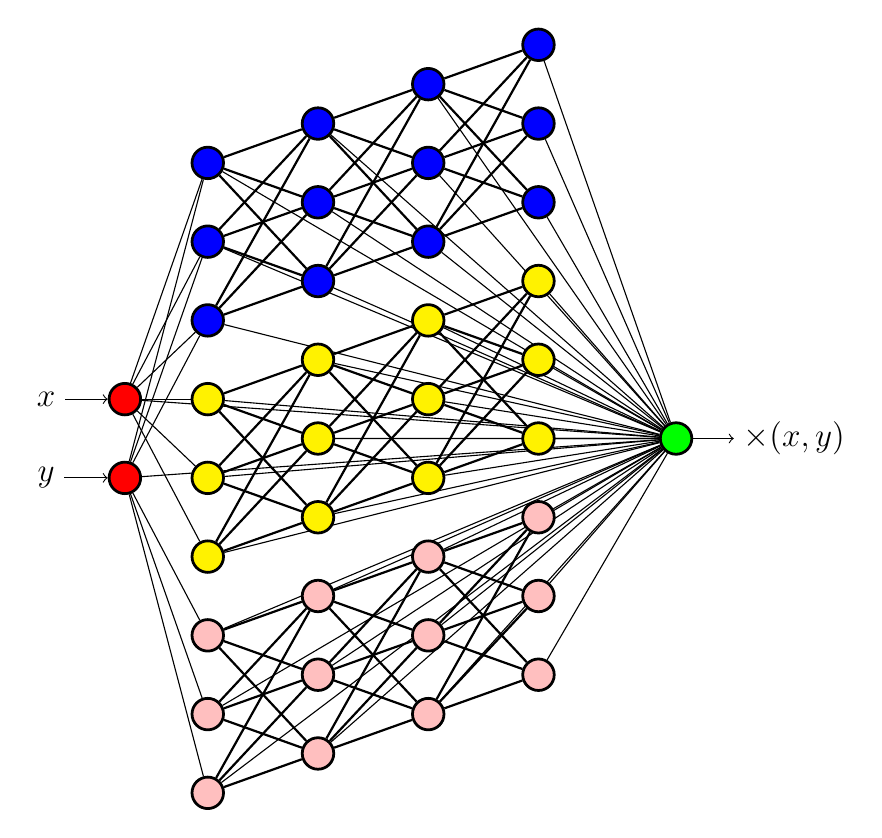
\begin{tikzpicture}
    \node [neuron, draw = black, fill = red] (input1) at (0,0) {} ;
    \node [neuron, below of = input1, draw = black, fill = red] (input2) {} ;
    \node [neuron, right of = input1, yshift = 3cm, xshift = 1.5, fill=blue] (hiddenA11) {};
    \node [neuron, below of = hiddenA11, yshift = 0cm, fill=blue] (hiddenA12) {};
    \node [neuron, below of = hiddenA12, yshift = 0cm, fill=blue] (hiddenA13) {};

    \node [neuron, right of = hiddenA11, yshift = 0.5cm, xshift = .4cm, fill=blue] (hiddenA21) {};
    \node [neuron, below of = hiddenA21, yshift = 0cm, fill=blue] (hiddenA22) {};
    \node [neuron, below of = hiddenA22, yshift = 0cm, fill=blue] (hiddenA23) {};

    \node [neuron, right of = hiddenA21, yshift = 0.5cm, xshift = .4cm, fill=blue] (hiddenA31) {};
    \node [neuron, below of = hiddenA31, yshift = 0cm, fill=blue] (hiddenA32) {};
    \node [neuron, below of = hiddenA32, yshift = 0cm, fill=blue] (hiddenA33) {};

    \node [neuron, right of = hiddenA31, yshift = 0.5cm, xshift = .4cm, fill=blue] (hiddenA41) {};
    \node [neuron, below of = hiddenA41, yshift = 0cm, fill=blue] (hiddenA42) {};
    \node [neuron, below of = hiddenA42, yshift = 0cm, fill=blue] (hiddenA43) {};

    \node [neuron, right of = input1, yshift = 0cm, xshift = 1.5, fill=yellow] (hiddenB11) {};
    \node [neuron, below of = hiddenB11, yshift = 0cm, fill=yellow] (hiddenB12) {};
    \node [neuron, below of = hiddenB12, yshift = 0cm, fill=yellow] (hiddenB13) {};
    \node [neuron, right of = hiddenB11, yshift = 0.5cm, xshift = .4cm, fill=yellow] (hiddenB21) {};
    \node [neuron, below of = hiddenB21, yshift = 0cm, fill=yellow] (hiddenB22) {};
    \node [neuron, below of = hiddenB22, yshift = 0cm, fill=yellow] (hiddenB23) {};
    \node [neuron, right of = hiddenB21, yshift = 0.5cm, xshift = .4cm, fill=yellow] (hiddenB31) {};
    \node [neuron, below of = hiddenB31, yshift = 0cm, fill=yellow] (hiddenB32) {};
    \node [neuron, below of = hiddenB32, yshift = 0cm, fill=yellow] (hiddenB33) {};
    \node [neuron, right of = hiddenB31, yshift = 0.5cm, xshift = .4cm, fill=yellow] (hiddenB41) {};
    \node [neuron, below of = hiddenB41, yshift = 0cm, fill=yellow] (hiddenB42) {};
    \node [neuron, below of = hiddenB42, yshift = 0cm, fill=yellow] (hiddenB43) {};

    \node [neuron, right of = input1, yshift = -3cm, xshift = 1.5, fill=pink] (hiddenC11) {};
    \node [neuron, below of = hiddenC11, yshift = 0cm, fill=pink] (hiddenC12) {};
    \node [neuron, below of = hiddenC12, yshift = 0cm, fill=pink] (hiddenC13) {};
    \node [neuron, right of = hiddenC11, yshift = 0.5cm, xshift = .4cm, fill=pink] (hiddenC21) {};
    \node [neuron, below of = hiddenC21, yshift = 0cm, fill=pink] (hiddenC22) {};
    \node [neuron, below of = hiddenC22, yshift = 0cm, fill=pink] (hiddenC23) {};
    \node [neuron, right of = hiddenC21, yshift = 0.5cm, xshift = .4cm, fill=pink] (hiddenC31) {};
    \node [neuron, below of = hiddenC31, yshift = 0cm, fill=pink] (hiddenC32) {};
    \node [neuron, below of = hiddenC32, yshift = 0cm, fill=pink] (hiddenC33) {};
    \node [neuron, right of = hiddenC31, yshift = 0.5cm, xshift = .4cm, fill=pink] (hiddenC41) {};
    \node [neuron, below of = hiddenC41, yshift = 0cm, fill=pink] (hiddenC42) {};
    \node [neuron, below of = hiddenC42, yshift = 0cm, fill=pink] (hiddenC43) {};

    \node [neuron, right of = input1, yshift = -.5cm, xshift = 6cm, draw = black, fill = green] (output) {};

    \begin{pgfonlayer}{bg} % background layer
    \draw (input1) -- (output);
    \draw (input2) -- (output);
    \foreach \m in {1,2,3}
        {
        \draw (input1) -- (hiddenA1\m);
        \draw (input2) -- (hiddenA1\m);
        \draw (input1) -- (hiddenB1\m);
        \draw (input2) -- (hiddenC1\m);
        \foreach \l in {A,B,C}
            {
            \draw (hidden\l1\m) -- (output);
            \draw (hidden\l2\m) -- (output);
            \draw (hidden\l3\m) -- (output);
            \draw (hidden\l4\m) -- (output);
            \foreach \k in {1,2,3}
                {
                \draw[thick] (hidden\l1\m) -- (hidden\l2\k);
                \draw[thick] (hidden\l2\m) -- (hidden\l3\k);
                \draw[thick] (hidden\l3\m) -- (hidden\l4\k);
                }
            }
        }
    \end{pgfonlayer}
        
    \node [draw = none, left of = input1] (inputlabel1) {\large $x$};
    \draw [->] (inputlabel1) --  (input1);
    \node [draw = none, left of = input2] (inputlabel2) {\large $y$};
    \draw [->] (inputlabel2) --  (input2);
    \node [draw = none, right of = output, xshift = .5cm] (outputlabel) {\large $\times(x,y)$};
    \draw [->] (output) --  (outputlabel);
    \end{tikzpicture}
    }%
    % \caption{.}
    % \label{.}
\end{figure}

\tikzset{neuron/.style={circle,draw,minimum size=4mm,line width = 1pt},neuron missing/.style={draw=none, scale=1.5,text height=2mm,execute at begin node=\color{black}$\vdots$},block/.style={rectangle,draw,minimum size=1cm,line width = 1pt},block missing/.style={draw=none,scale=1.5,text height=2mm,execute at begin node=\color{black}$\ddots$}}
\begin{figure}[H]
    \centering
    \resizebox{0.75\textwidth}{!}{%
    \begin{tikzpicture}
    \node [neuron, draw = black, fill = red] (input1) at (0,0) {} ;
    \node [neuron, below of = input1, draw = black, fill = red] (input2) {} ;
    \node [neuron, below of = input2, draw = black, fill = red] (input3) {} ;
    \node [neuron, below of = input3, draw = black, fill = red] (input4) {} ;
    \node [neuron missing, below of = input4] (inputMissing) {} ;
    \node [neuron, below of = inputMissing, draw = black, fill = red] (inputd) {} ;

    \node [block, right of = input2, yshift = 0cm, xshift = 1cm, fill=white] (block1) {\large $\hat{\times}$};
    \node [block, right of = input3, yshift = 0cm, xshift = 3cm, fill=white] (block2) {\large $\hat{\times}$};
    \node [block, right of = input4, yshift = 0cm, xshift = 5cm, fill=white] (block3) {\large $\hat{\times}$};
    \node [block missing, right of = block3, yshift = -.8cm, fill=white] (blockMissing) {};
    \node [block, right of = inputd, yshift = 0cm, xshift = 8cm, fill=white] (blockd) {\large $\hat{\times}$};
    
    \node [neuron, right of = blockd, xshift = .5cm, draw = black, fill = green] (output) {};

    \begin{pgfonlayer}{bg} % background layer
    \draw[thick] (input1) -- (block1);
    \draw[thick] (input2) -- (block1);
    \draw[thick] (block1) -- (block2);
    \draw[thick] (input3) -- (block2);
    \draw[thick] (block2) -- (block3);
    \draw[thick] (input4) -- (block3);
    \draw[thick] (block3) -- (blockMissing);
    \draw[thick] (inputd) -- (blockd);
    \draw[thick] (blockMissing) -- (blockd);
    \draw[thick] (blockd) -- (output);
    \end{pgfonlayer}
        
    \node [draw = none, left of = input1] (inputlabel1) {\large $x_1$};
    \draw [->] (inputlabel1) --  (input1);
    \node [draw = none, left of = input2] (inputlabel2) {\large $x_2$};
    \draw [->] (inputlabel2) --  (input2);
    \node [draw = none, left of = input3] (inputlabel3) {\large $x_3$};
    \draw [->] (inputlabel3) --  (input3);
    \node [draw = none, left of = input4] (inputlabel4) {\large $x_4$};
    \draw [->] (inputlabel4) --  (input4);
    \node [draw = none, left of = inputd] (inputlabeld) {\large $x_d$};
    \draw [->] (inputlabeld) --  (inputd);
    \node [draw = none, right of = output, xshift = 1cm] (outputlabel) {\large $\Pi(x_1,\dots,x_d)$};
    \draw [->] (output) --  (outputlabel);
    \end{tikzpicture}
    }%
    % \caption{.}
    % \label{.}
\end{figure}

\tikzset{neuron/.style={circle,draw,minimum size=4mm,line width = 1pt},neuron missing/.style={draw=none, scale=1.5,text height=2mm,execute at begin node=\color{black}$\vdots$},block/.style={rectangle,draw,minimum size=1cm,line width = 1pt},block missing/.style={draw=none,scale=1.5,text height=2mm,execute at begin node=\color{black}$\ddots$}}
\begin{figure}[H]
    \centering
    \resizebox{0.5\textwidth}{!}{%
    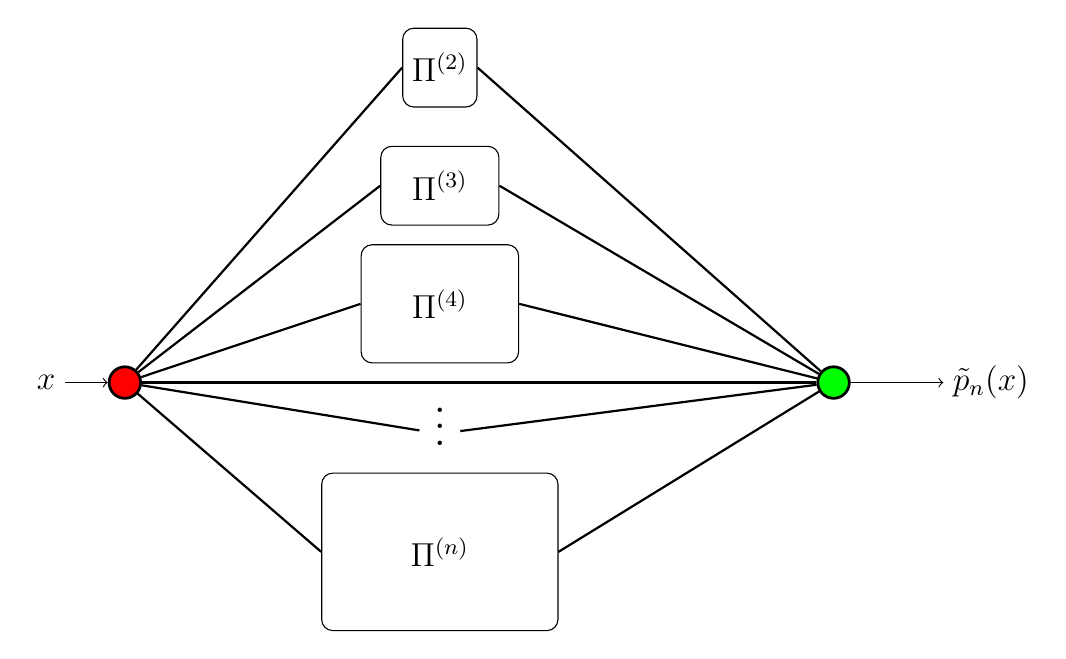
\begin{tikzpicture}
    \node [neuron, draw = black, fill = red] (input1) at (0,0) {} ;

    \node [block, right of = input1, yshift = 4cm, xshift = 3cm, fill=white] (block1) {\large $\Pi^{(2)}$};
    \node [block, minimum width=1.5cm, text centered, align = center, below of = block1, yshift = -.5cm, fill=white] (block2) {\large $\Pi^{(3)}$};
    \node [block, minimum width=2cm, minimum height=1.5cm, text centered, align = center, below of = block2, yshift = -.5cm, fill=white] (block3) {\large $\Pi^{(4)}$};
    \node [neuron missing, below of = block3, yshift = -0.1cm, fill=white] (blockMissing) {};
    \node [block, minimum width=3cm, minimum height=2cm, text centered, align = center, below of = blockMissing, yshift = -.5cm,  fill=white] (blockk) {\large $\Pi^{(n)}$};
    
    \node [neuron, right of = input1, xshift = 8cm, draw = black, fill = green] (output) {};

    \begin{pgfonlayer}{bg} % background layer
    \draw[thick] (input1) -- (block1.west);
    \draw[thick] (input1) -- (block2.west);
    \draw[thick] (input1) -- (block3.west);
    \draw[thick] (input1) -- (blockMissing);
    \draw[thick] (input1) -- (blockk.west);

    \draw[thick] (input1) -- (output);
    \draw[thick] (block1.east) -- (output);
    \draw[thick] (block2.east) -- (output);
    \draw[thick] (block3.east) -- (output);
    \draw[thick] (blockMissing) -- (output);
    \draw[thick] (blockk.east) -- (output);
    \end{pgfonlayer}
        
    \node [draw = none, left of = input1] (inputlabel1) {\large $x$};
    \draw [->] (inputlabel1) --  (input1);
    \node [draw = none, right of = output, xshift = 1cm] (outputlabel) {\large $\tilde{p}_n(x)$};
    \draw [->] (output) --  (outputlabel);
    \end{tikzpicture}
    }%
    % \caption{.}
    % \label{.}
\end{figure}

\tikzset{neuron/.style={circle,draw,minimum size=4mm,line width = 1pt},neuron missing/.style={draw=none, scale=1.5,text height=2mm,execute at begin node=\color{black}$\vdots$},block/.style={rectangle,draw,minimum size=1cm,line width = 1pt},block missing/.style={draw=none,scale=1.5,text height=2mm,execute at begin node=\color{black}$\ddots$}}
\begin{figure}[H]
    \centering
    \resizebox{.9\textwidth}{!}{%
    \begin{tikzpicture}
    \node [neuron, draw = black, fill = red] (input1) at (0,0) {} ;
    \node [neuron, below of = input1, draw = black, fill = red] (input2) {} ;
    \node [neuron, below of = input2, draw = black, fill = red] (input3) {} ;
    \node [neuron missing, below of = input3] (inputMissing) {} ;
    \node [neuron, below of = inputMissing, draw = black, fill = red] (inputd) {} ;

    \node [block, right of = input1, yshift = 4cm, xshift = 3cm, fill=white] (block1A) {\large $\Pi^{(i_1)}$};
    \node [block, minimum width=1.2cm, text centered, align = center, below of = block1A, yshift = 0cm, fill=white] (block2A) {\large $\Pi^{(i_2)}$};
    \node [block, minimum width=1.5cm, minimum height=1cm, text centered, align = center, below of = block2A, yshift = 0cm, fill=white] (block3A) {\large $\Pi^{(i_3)}$};
    \node [neuron missing, below of = block3A, yshift = .35cm, fill=white] (blockMissingA) {};
    \node [block, minimum width=2cm, minimum height=1.5cm, text centered, align = center, below of = blockMissingA, yshift = 0cm,  fill=white] (blockkA) {\large $\Pi^{(i_d)}$};
    
    \node [neuron missing, below of = blockkA, yshift = -0.1cm, fill=white] (blockMissingAB) {};
    \node [neuron missing, below of = blockMissingAB, yshift = -0.1cm, fill=white] (blockMissingAB2) {};

    \node [block, below of = blockMissingAB2, yshift = 0cm, xshift = 0cm, fill=white] (block1B) {\large $\Pi^{(j_1)}$};
    \node [block, minimum width=1.2cm, text centered, align = center, below of = block1B, yshift = 0cm, fill=white] (block2B) {\large $\Pi^{(j_2)}$};
    \node [block, minimum width=1.5cm, minimum height=1cm, text centered, align = center, below of = block2B, yshift = 0cm, fill=white] (block3B) {\large $\Pi^{(j_3)}$};
    \node [neuron missing, below of = block3B, yshift = 0.35cm, fill=white] (blockMissingB) {};
    \node [block, minimum width=2cm, minimum height=1.5cm, text centered, align = center, below of = blockMissingB, yshift = 0cm,  fill=white] (blockkB) {\large $\Pi^{(j_d)}$};

    \node [block, right of = block2A, yshift = 0cm, xshift = 1cm, fill=white] (times1A) {\large $\hat{\times}$};
    \node [block, right of = block3A, yshift = 0cm, xshift = 3cm, fill=white] (times2A) {\large $\hat{\times}$};
    \node [block missing, right of = blockMissingA, yshift = 0cm, xshift = 3.5cm, fill=white] (timesMissingA) {};
    \node [block, right of = blockkA, yshift = 0cm, xshift = 8cm, fill=white] (timesdA) {\large $\hat{\times}$};

    \node [block, right of = block2B, yshift = 0cm, xshift = 1cm, fill=white] (times1B) {\large $\hat{\times}$};
    \node [block, right of = block3B, yshift = 0cm, xshift = 3cm, fill=white] (times2B) {\large $\hat{\times}$};
    \node [block missing, right of = blockMissingB, yshift = 0cm, xshift = 3.5cm, fill=white] (timesMissingB) {};
    \node [block, right of = blockkB, yshift = 0cm, xshift = 8cm, fill=white] (timesdB) {\large $\hat{\times}$};

    \node [neuron, right of = inputMissing, xshift = 15cm, draw = black, fill = green] (output) {};

    \begin{pgfonlayer}{bg} % background layer
    \foreach \m in {A,B}
        {
        \draw[thick] (input1) -- (block1\m.west);
        \draw[thick] (input2) -- (block2\m.west);
        \draw[thick] (input3) -- (block3\m.west);
        \draw[thick] (inputd) -- (blockk\m.west);

        \draw[thick] (block1\m.east) -- (times1\m);
        \draw[thick] (block2\m.east) -- (times1\m);
        \draw[thick] (times1\m.east) -- (times2\m);
        \draw[thick] (block3\m.east) -- (times2\m);
        \draw[thick] (times2\m.east) -- (timesMissing\m);
        \draw[thick] (timesMissing\m) -- (timesd\m);
        \draw[thick] (blockk\m.east) -- (timesd\m);

        \draw[thick] (timesd\m.east) -- (output);
        }
    
    

    \draw[thick] (timesdA.east) -- (output);

    \end{pgfonlayer}
    
        
    \node [draw = none, left of = input1] (inputlabel1) {\large $x_1$};
    \draw [->] (inputlabel1) --  (input1);
    \node [draw = none, left of = input2] (inputlabel2) {\large $x_2$};
    \draw [->] (inputlabel2) --  (input2);
    \node [draw = none, left of = input3] (inputlabel3) {\large $x_3$};
    \draw [->] (inputlabel3) --  (input3);
    \node [draw = none, left of = inputd] (inputlabeld) {\large $x_d$};
    \draw [->] (inputlabeld) --  (inputd);
    \node [draw = none, right of = output, xshift = 1cm] (outputlabel) {\large $\tilde{q}_n(x_1,\dots,x_d)$};
    \draw [->] (output) --  (outputlabel);
    \end{tikzpicture}
    }%
    % \caption{.}
    % \label{.}
\end{figure}





\end{document}